%Bojan nestorovic

\section{Deployment}

Postoje mnogi dodaci koji se koriste da prebace build fajlove posle uspesnog kompajliranja na željenu lokaciju ili web server. Ovde ćemo to pokazati na primeru "Deploy to container Plugin". 


Da bi se instalirao taj dodatak, potrebno je otići na Jenkins -> Manage Plugins, pronađete željeni dodatak i instalirate ga. Posle toga je potrebno restartovati jenkins server. 
\begin{figure}
\begin{center}
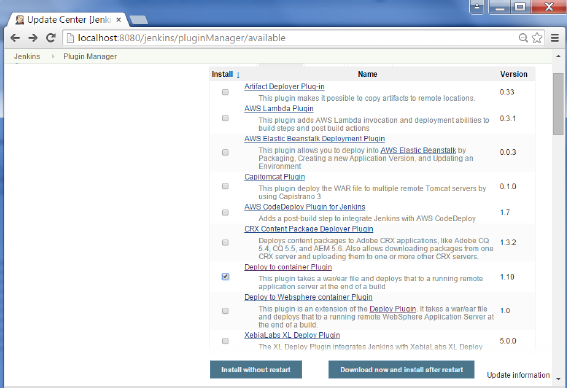
\includegraphics[scale=0.45]{slike/deploy_to_container_plugin.png}
\end{center}
\caption{Dodavanje dodatka}
\label{fig:deploy_to_container_plugin}
\end{figure}






%\subsection{podnaslov}


